% Normal text
\begin{frame}[c]{...}
  \begin{itemize}
    \item ...
  \end{itemize}
\end{frame}

% Text in two columns
\begin{frame}[c]{...}
  \begin{columns}
    \column{.45\textwidth}
        \begin{itemize}
            \item ...
        \end{itemize}
    \column{.45\textwidth}
    \begin{itemize}
        \item ...
    \end{itemize}
  \end{columns}
\end{frame}

% Just a table
\begin{frame}[c]{...}
    \centering
    \begin{tabular}{cccc}
      \toprule
      ... & ... & ... & ...\\
      \midrule
      ... & ... & ... & ...\\
      \bottomrule
    \end{tabular}
\end{frame}

% Two columns with an image
\begin{frame}[c]{...}
    \begin{columns}
    \column{.45\textwidth}
        \begin{itemize}
            \item ...
        \end{itemize}
    \column{.45\textwidth}
    \centering
    \includegraphics[
        width=\linewidth,
        height=.8\textheight,
        keepaspectratio
        ]{img/...}
    \end{columns}
\end{frame}

% Two columns with Stanli
\begin{frame}[c]{...}
    \begin{columns}
    \column{.45\textwidth}
        \begin{itemize}
            \item ...
        \end{itemize}
    \column{.45\textwidth}
    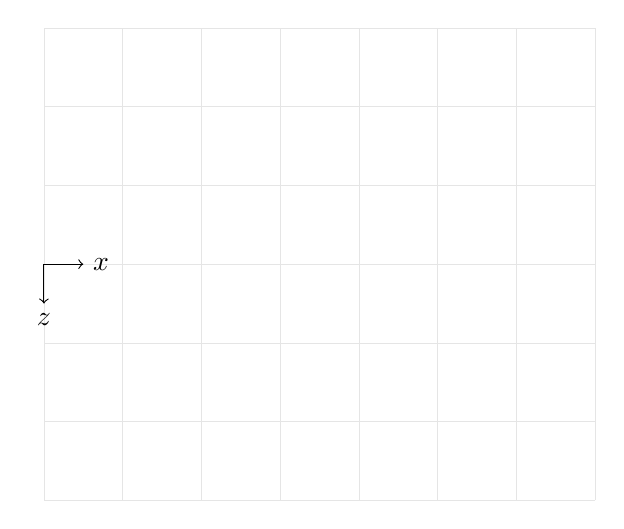
\begin{tikzpicture}
            \draw[help lines, gray!20, step=1] (0, 0) grid (7,6); % To simplify construction
            \draw[->] (0,3) -- (.5,3) node[right] {$x$};
            \draw[->] (0,3) -- (0,2.5) node[below] {$z$};
        \end{tikzpicture}
\end{frame}

% Two columns with a TikZ (flowchart)
\begin{frame}[c]{...}
  \begin{columns}
    \column{.45\textwidth}
    \begin{itemize}
        \item ...
    \end{itemize}
    
    \column{.45\textwidth}
      \centering
      \begin{tikzpicture}[
        node distance=0.5cm,
        box/.style={draw,rectangle,minimum width=4cm,minimum height=0.8cm,align=center},
        arrow/.style={->,>=stealth}]

        % Nodes
        \node[box, below=of data] (analytical) {
            Calcul analytique
        };
        \node[box, below=of analytical] (fem) {
            Simulation FEM
        };

        % Arrows
        \draw[arrow] (analytical) -- (fem);
    \end{tikzpicture}
  \end{columns}
\end{frame}

% How to cite
\cite{...} % with name

% How to put bibliography in the slides
\printbibliography

% If you have some references that are not cited in the slides, but you want to include them in the bibliography, use this before \printbibliography
\nocite{*}

% Warning 
\item[\textcolor{orange}{\faExclamationTriangle}]

% For colors in bullet list
\item[$\textcolor{red}{\bullet}$]
\item[$\textcolor{green}{\bullet}$]
\item[$\textcolor{blue}{\bullet}$]
\item[$\textcolor{yellow}{\bullet}$]

% To list attached files
\item[\textcolor{black}\faFileArchive] .wbpz:
\item[\textcolor{black}\faFilePdf] .pdf: 
\item[\textcolor{black}\faFolder] folder:
\item[\textcolor{black}\faFileExcel] .xlsx:
\item[\textcolor{black}\faFileCode] .py: 
\item[\textcolor{black}\faFile] .txt: 
\item[\textcolor{black}\faImage] img.png: 
\item[\textcolor{black}\faChartBar] plot.png: 
% Not bad also \faTable or \faCalculator